\documentclass[11pt]{article}

\usepackage[margin=1in]{geometry}
\usepackage{amsfonts, amsmath, amssymb}
\usepackage[none]{hyphenat}
\usepackage{fancyhdr}
\usepackage{graphicx}
\usepackage{float}
\usepackage[nottoc, notlot, notlof]{tocbibind}
\usepackage{hyperref}

\pagestyle{fancy}
\fancyhead{}
\fancyfoot{}
\fancyhead[L]{\slshape \MakeUppercase{Cassette deck}}
\fancyhead[R]{\slshape Implementation}
\fancyfoot[C]{\thepage}
\renewcommand{\footrulewidth}{0pt}

\parindent 0ex %
\renewcommand{\baselinestretch}{1.5}

\begin{document}

\begin{titlepage}
\begin{center}
\vspace*{1cm}
\Large{\textbf{Software Engineering}}\\
\Large{\textbf{Modeling and Implementation Project}}
\vfill
\line(1,0){400}\\[1mm]
\huge{\textbf{“Simulator of a Cassette Deck”}}\\[3mm]
\Large{\textbf{- Implementation -}}\\[1mm]
\line(1,0){400}\\
\vfill
By Constant Théo and Essafsyfy Abdelkrim\\
Academic year 2018-2019
\end{center}
\end{titlepage}

\tableofcontents
\thispagestyle{empty}
\clearpage
\setcounter{page}{1}

\section{Implementation choices}
\label{sec:implChoices}
\subsection{\textit{Scene Builder}}
\begin{center}

\includegraphics[width=2cm]{./img/SceneBuilder.png}\\
\end{center}
For not only the modeling but also the implementation phase of the project, we have used \textit{Scene Builder} to design the \textit{JavaFx GUI}.\\
\textit{FXML} files were generated and introduced to our project.
\subsection{\textit{Maven}}
\begin{center}

\includegraphics[width=2.5cm]{./img/maven.png}\\
\end{center}
We have chosen \textit{maven} to easily manage jar files and organize the project.
\subsection{\textit{IDE}s}
\begin{center}
\includegraphics[width=2.5cm]{./img/netBeans.png} \& 
\includegraphics[width=5cm]{./img/eclipse.png}
\end{center}
To be sure the application is \textit{IDE}-independent, we have used each a different java \textit{IDE}, \textit{Netbeans} and \textit{Eclipse}. It is note worthy that we have encountered some behavioral differences caused by these \textit{IDEs}, noticeably, the path each one uses to acces the \textit{fxml} files.
\subsection{\textit{MVC}}
\begin{center}
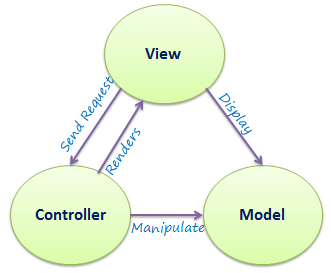
\includegraphics[width=5cm]{./img/mvc.png}
\end{center}
We have tried to use as best we could the Model, View, Controler architecture, the project uses 2 of the 3 packages, "model" and "controller", for the "view" we have encountered -as said above- differences between the \textit{IDE}s which forced us to place the \textit{fxml} files in the src/main/resources folder.

\section{Modeling differences}
There have been some changes to the model since its conception in the \textbf{Modeling Report}, notably:
\begin{itemize}
\item The use of \textit{GridPaneLayout} and \textit{H/VBoxes }to contain the different nodes.
\item In the Launcher, the function "Built-in microphone" is no longer disabled if the "Audio recorder functionality" isn't checked, also, a "Music detection"\textit{checkbox} has been added.
\begin{center}
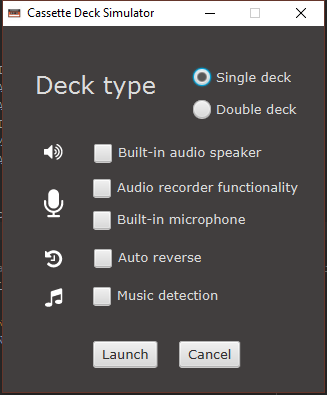
\includegraphics[width=5cm]{./img/deckLauncher.png}\\
\end{center}
\item  In case of a double deck, the functionality is split to two decks instead of "Player" and "Recorder" in the previous model.
\item Added missing \textit{Previous/Next} Song, \textit{Flip Cassette} and \textit{Source} -if the deck has a built-in audio Speaker- buttons.
\begin{center}
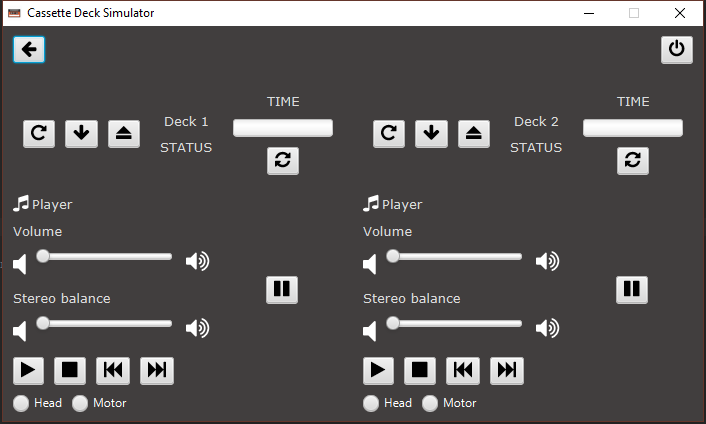
\includegraphics[width=10cm]{./img/doubleDeck_noF.png}\\
\end{center}
\item Replaced buttons' text with icons and a mouse-over tooltip to display their name.
\item Removed "Remove cassette" button, due to its redundancy with the Eject button. In this simulation, ejecting the cassette holder and removing the cassette within are both done by clicking the "Eject" button.
\item "Pause" button is now centered between the "Player" and "Recorder".

\end{itemize}

%\pagebreak
\section{Design Patterns}
For this application, we implemented the "state machine" design pattern to handle the different states of the Deck class. Indeed, the deck (s) of the device will not have the same behavior at the start of a button depending on the state in which they are (s). A deck can be turned off, on hold, playing, fast-forwarding, fast-rewinding, or recording. We have chosen not to make a pause state, because, in our opinion, it simply is a possible action when the deck is in the reading or recording state. The pause button is a button that can be held down at the same time as the others, and can be engaged at any time. This is not the case for other buttons that disengage themselves when pressing another button (other than pause), and that can not be engaged at any time.
The state machine consists of a State interface that inherits each possible state. The class that can take these states (Deck in this case) has a State attribute and the behavior of all Deck methods that are likely to vary by state is delegated to State. This State object will change each time the state changes, thus another class will take care of Deck's behavior.
%\pagebreak
\section{Known Issues}
\begin{itemize}
\item JUnit tests have not been completed.
\end{itemize}
%\pagebreak
\section{Miscellaneous}
\subsection{\textit{Git}}
Throughout the project, we have used version control \textit{git} and \textit{github} to organize and avoid conflicts while working on the project. After receiving feedback from the modeling report, we have decided to make the repository private. We invite you to send a contribution request to either $\href{mailto:remagkes@gmail.com}{remagkes@gmail.com} $ or $\href{mailto:to.constant@gmail.com}{to.constant@gmail.com}$
\subsection{Video link}
As asked in the requisites, a video demonstrating the basic features of the simulation can be accessed via this link: 



\end{document}
